\documentclass{beamer}

\usepackage[utf8]{inputenc}
\usepackage[T1]{fontenc}
\usepackage{textpos}
\usepackage{tikz}

\usetheme{Madrid}
\usecolortheme{beaver}

% Custom changes:
\setbeamertemplate{footline}[frame number]{}
\definecolor{university_tuebingen}{RGB}{165,30,55}
\setbeamercolor{frametitle}{fg=university_tuebingen, bg=white}
\setbeamercolor{title}{fg=university_tuebingen}

\addtobeamertemplate{frametitle}{}{
\begin{tikzpicture}[remember picture, overlay]
\node[anchor=north east,yshift=0cm] at (current page.north east)
{
\includegraphics[width=3cm]{../common/logo_uni_tuebingen2.png}};
\end{tikzpicture}}



\author{Prof. Dr. Christiane Zarfl, Dipl.-Inf. Willi Kappler}
%\date{\today}
\date{}
%\institute{Universität Tübingen}
\institute{}


\matlabTitle{2. Der Editor und Grafikplots}

% Rechtschreibprüfung mit: aspell -l de -t --tex-check-comments -c lecture2/lecture2.tex

\setcounter{mchapter}{2}
\setcounter{mexercise}{0}

\begin{document}
  {
\beamertemplatenavigationsymbolsempty % suppress navigation on this (= first) slide
\begin{frame}[plain] % plain means: no header and footer on this (= first) slide
    \begin{textblock*}{0cm}(0.5cm, -0.7cm)
        
\includegraphics[width=11.0cm]{../common/logo_uni_tuebingen.png}
    \end{textblock*}
    \titlepage
    \begin{textblock*}{0cm}(0.1cm, -2.5cm)
        \textcolor{university_tuebingen}{\rule{11.8cm}{0.2cm}}
    \end{textblock*}
\end{frame}
}


    \section{Einleitung}

    \subsection{Motivation}
    \begin{frame}
        \frametitle{Sie wissen bereits...}
        \begin{itemize}
            \item wie Sie in Matlab Variablen definieren und damit Werte wiederverwenden können.
            \item wie Sie in Matlab mit Vektoren rechnen und damit effizient auch große Datenmengen verarbeiten können.
        \end{itemize}

        \vspace{0.3cm}

        \textit{Wie kann man mehrere Rechenschritte/Matlab-Befehle, die häufig benötigt werden, ``speichern'' und zusammenfassen?} \\

        \vspace{0.3cm}

        \textbf{Nach diesem zweiten Block...} \\

        \vspace{0.3cm}

        \begin{itemize}
            \item können Sie eigene Script Files erstellen (Bsp. 1D-Stofftransport- gleichung)
            \item können Sie x-y Plots erstellen, bearbeiten und speichern.
        \end{itemize}
    \end{frame}


    \subsection{Script Files}
    \begin{frame}
        \frametitle{Programme Schreiben mit Matlab - Script Files}
        \begin{itemize}
            \item Matlab ist mehr als nur ein Taschenrechner.
            \item Ein Script-File ist eine Aneinanderreihung von Matlab-Befehlen.
            \item Matlab-Scripts haben die Dateiendung ``\texttt{.m}''.
            \item Bsp.: Ihr Programm heißt \texttt{MeinScript.m} und befindet sich im Verzeichnis \texttt{MyDocuments\textbackslash ich\textbackslash Matlab}.
            \item Dieser Pfad muss das gegenwärtige \textbf{Arbeitsverzeichnis} von Matlab sein.
            \item Dann führt der Befehl \matlabInput{MeinScript} (ohne Dateiendung) im ``Command Window'' den Inhalt des Scriptes aus.
            \item Dateinamen dürfen keine Sonderzeichen oder Leerzeichen enthalten und auch nicht mit Ziffern anfangen.
            \item Script Files/Programme können mit jedem Texteditor oder mit dem Matlab-eigenen Editor erstellt werden.
          \end{itemize}
      \end{frame}

      \subsection{Matlab Editor}
      \begin{frame}
          \frametitle{Der Matlab Editor}
          \begin{itemize}
              \item Legen Sie ein Verzeichnis für die heutige Übung an.
              \item Machen Sie dies zum aktiven Verzeichnis von Matlab.
              \item Aufruf des Editors vom prompt: \matlabInput{\matlabLink{edit} dateiname}.
              \item \alert{Achtung}: Kommentieren Sie \textbf{immer} Ihre Scripte: Kommentare beginnen mit \matlabInput{\%} und enden mit dem Zeilenende.
          \end{itemize}

          \begin{figure}
            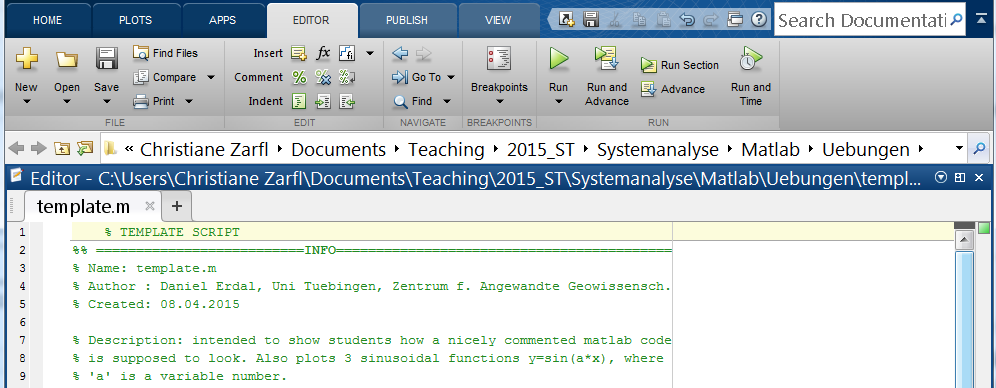
\includegraphics[width=10.0cm]{matlab_gui.png}
          \end{figure}
      \end{frame}

      \section{Plots}

      \subsection{XY-Plots}
      \begin{frame}
          \frametitle{XY-Plots}

          \vspace{-0.5cm}

          \begin{itemize}
              \item \matlabInput{\matlabLink{plot}} trägt numerische Daten gegeneinander auf (\matlabInput{doc \matlabLink{plot}}).
              \item \matlabInput{\matlabLink{plot}(x,y)} erzeugt ein Grafikfenster (\texttt{``figure''}) indem die Werte \texttt{y} gegen \texttt{x} aufgetragen sind.
              \item Beispiel: die Wurzelfunktion im Intervall [0,6] zeichnen:
              % \item \matlabInput{x = 0:0.5:6; y = sqrt(x); \matlabLink{plot}(x,y)}
              \insertMatlabOnlyCode[lastline=1]{example2_1}
          \end{itemize}

          \vspace{-0.3cm}

          \begin{figure}
              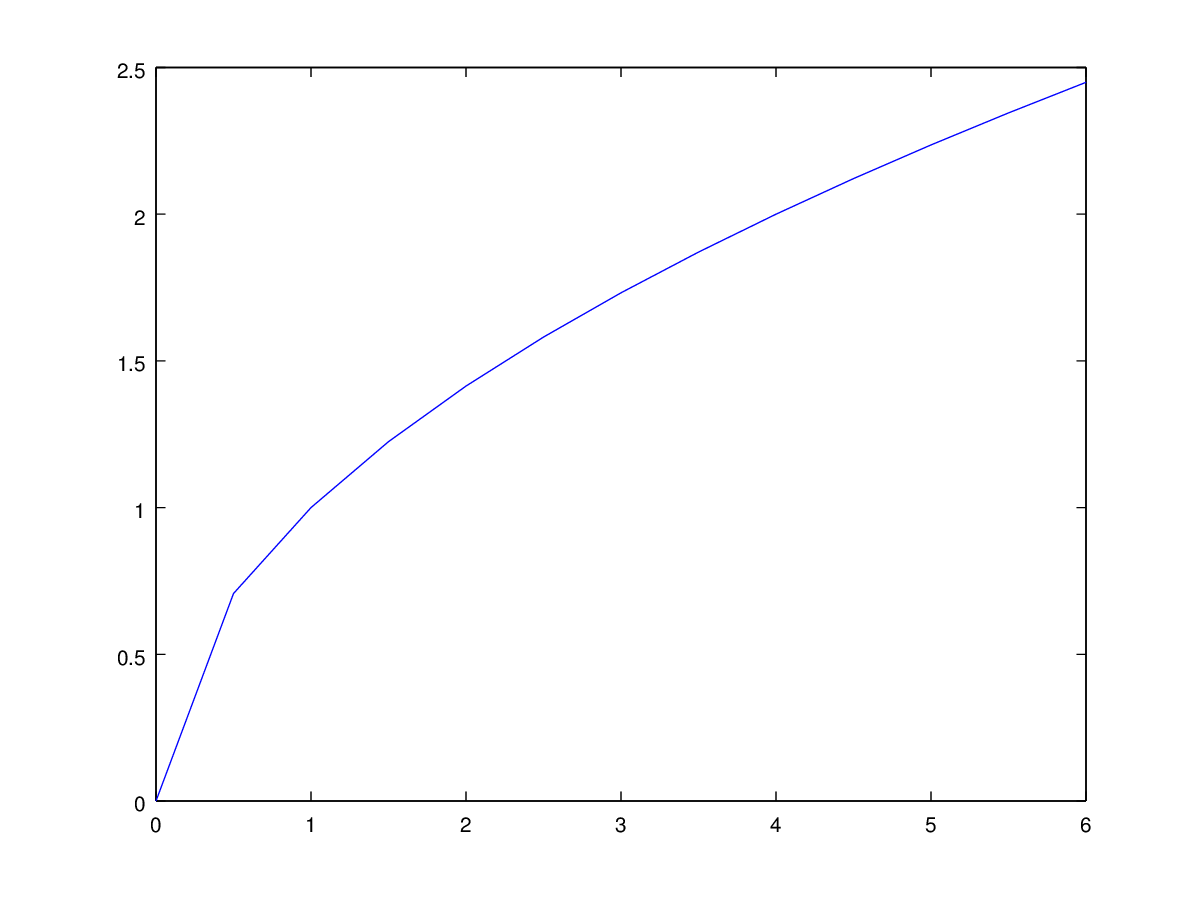
\includegraphics[width=7.0cm]{example2_1.png}
          \end{figure}
      \end{frame}

      \secMexercise
      \begin{frame}
          \frameMexercise
          \begin{exercise}
              \sloppy
              Schreiben Sie ein Script (\texttt{Wurzel.m}), welches die auf der letzten Folie gezeigte Grafik erzeugt.\\ \\

              \textbf{Tipp}: Der erste Befehl eines Scripts sollte \texttt{clear all} sein, um den Arbeitsspeicher zu leeren\\ \\

              Ändern Sie die Auflösung der x-Achse.
          \end{exercise}
      \end{frame}

      \secMexercise
      \begin{frame}
          \frameMexercise
          \begin{exercise}
              \sloppy
              Die eindimensionale Stoffverteilung bei pulsartiger Zugabe des Stoffes hat die analytische Lösung:

              \begin{displaymath}
                  c(t,x) = \frac{1}{\sqrt{4 \pi Dt}} exp \left( - \frac{(x-vt)^{2}}{4Dt} \right)
              \end{displaymath}

              \vspace{0.5cm}

              Schreiben Sie ein Script, welches die räumliche Stoffverteilung graphisch darstellt. (Fortsetzung nächste Folie)\\
          \end{exercise}
      \end{frame}

      \begin{frame}
          \frametitle{Fortsetzung}
          \begin{exercise}
              \sloppy
              Tips:

              \vspace{0.2cm}

              \begin{itemize}
                  \item Löschen sie zuerst den Arbeitsspeicher (\texttt{clear all})
                  \item Definieren sie die Parameter:
                  \begin{itemize}
                      \item \texttt{v}: Geschwindigkeit ($10^{-5} m/s$)
                      \item \texttt{D}: Diffusionskoeffizient ($10^{-7} m^{2}/s$)
                      \item \texttt{t}: Zeit (1 d = 86400 s)
                      \item \texttt{x}: Ortsvektor (0-2 m in 1cm-Schritten)
                  \end{itemize}
                  \item Berechnung der Konzentration (\texttt{c}, siehe Formel oben)
                  \item Plotten des Profils (\texttt{plot(x,c)})
              \end{itemize}

              \vspace{0.2cm}

              \alert{Erinnerung}: Bitte kommentieren Sie jede Zeile! Kommentare beginnen mit ``\texttt{\%}'' und enden mit dem Zeilenende.

          \end{exercise}
      \end{frame}

      \subsection{Plots schöner machen}
      \begin{frame}
          \frametitle{Plots schöner machen}

          \vspace{-1.0cm}

          \begin{itemize}
              \item Stilparameter in Hochkommata übergeben: \matlabInput{\matlabLink{plot}(x,c,'k:x');}
              \begin{itemize}
                  \item \matlabInput{k} $\Rightarrow$ schwarz; \matlabInput{:} $\Rightarrow$ gepunktete Linie; \matlabInput{x} $\Rightarrow$ x-Zeichen als Marker.
                  \item Informieren Sie sich mit \matlabInput{doc \matlabLink{plot}} über weitere Stilparameter.
              \end{itemize}
              \item Achsenbereiche festsetzen: \matlabInput{\matlabLink{xlim}([minx maxx]); \matlabLink{ylim}([miny maxy])}
              \item Achsenbeschriftung: \matlabInput{\matlabLink{xlabel}('x [m]');} und \matlabInput{\matlabLink{ylabel}('c [mol/L]');}.
              \item Titel hinzufügen: \matlabInput{\matlabLink{title}('Titeltext');}
              \item Legende hinzufügen: \matlabInput{\matlabLink{legend}('c');}
              \item Matlab kennt rudimentäre LaTeX-Syntax für Strings: \matlabInput{\matlabLink{xlabel}('c [mol/m\string^3]')} ergibt hoch gestellte ``3'',
              \matlabInput{\matlabLink{title}('c\_\{cons\}')} ergibt tief gestelltes ``cons''
          \end{itemize}
      \end{frame}

      \begin{frame}
          \frametitle{Mehrere Graphen in einem Plot, \texttt{figure}}
          \begin{itemize}
              \item Variante 1: mehrere Parameterpärchen übergeben: \matlabInput{\matlabLink{plot}(t1,c1,'r-',t2,c2,'b:')}
              \item Variante 2: mit \matlabInput{\matlabLink{hold} on} in Hinzufügmodus wechseln (und mit \matlabInput{\matlabLink{hold} off} wieder raus):
              \begin{itemize}
                  \item \matlabInput{\matlabLink{plot}(t1,c1,'r-');}
                  \item \matlabInput{\matlabLink{hold} on; \matlabLink{plot}(t2,c2,‘b:‘); \matlabLink{hold} off}
              \end{itemize}
              \item Ein neues Grafikfenster wird mit dem Befehl \matlabInput{\matlabLink{figure}} erzeugt:
              \begin{itemize}
                  \item \matlabInput{\matlabLink{figure}(1)}, erzeugt das Grafikfenster 1
                  \item Man kann somit zwischen den Grafikfenstern ``springen''.
              \end{itemize}
          \end{itemize}
      \end{frame}


      \secMexercise
      \begin{frame}
          \frameMexercise
          \begin{exercise}
              \sloppy
              \begin{itemize}
                  \item Verschönern Sie Ihren Plot von vorhin:
                  \item Zeichen Sie die Konzentration in rot!
                  \item Beschriften Sie die Achsen!
                  \item Geben Sie dem Plot einen Titel!
                  \item Fügen sie eine Legende hinzu!
                  \item Plotten Sie mehrere Konzentrationsprofile in Ihrer Grafik, für \texttt{t = 1,2,3} Tage
                  \item ... vergessen Sie das \alert{Kommentieren} nicht!
              \end{itemize}
          \end{exercise}
      \end{frame}

      \subsection{Verteilung 2}
      \begin{frame}
          \frametitle{Stufenartige Zugabe der Konzentration}
          \begin{itemize}
              \item Konzentrationsverteilung bei stufenartiger Anfangsverteilung:
              \begin{displaymath}
                  c(x,t) = \frac{c_{ini}}{2} erfc \left( \frac{x-vt}{\sqrt{4Dt}} \right)
              \end{displaymath}
              \item \texttt{erfc} ist die komplementäre Fehlerfunktion (in etwa das Integral der Gauß-Funktion)
              \item Vermutung: könnte in Matlab \matlabInput{\matlabLink{erfc}} heißen (Testen Sie: \matlabInput{help \matlabLink{erfc}})
          \end{itemize}
      \end{frame}

      \secMexercise
      \begin{frame}
          \frameMexercise
          \begin{exercise}
              \sloppy
              \begin{itemize}
                  \item Plotten Sie mehrere Konzentrationsprofile bei stufenartiger Anfangsverteilung:
                  \item \texttt{v}: Geschwindigkeit ($10^{-5} m/s$)
                  \item \texttt{D}: Dispersionskoeffizient ($10^{-7} m^{2}/s$)
                  \item $\mathtt{c_{ini}}$: Anfangskonzentration (1 mg/L)
                  \item \texttt{t}: Zeit (0, 1, 2, 3 Tage)
                  \item \texttt{x}: Ortsvektor (-2 bis 5 m in 1cm-Schritten)
                  \item Speichern Sie Ihr Script und kommentieren Sie es!
              \end{itemize}
          \end{exercise}
      \end{frame}

      \subsection{Plots speichern}
      \begin{frame}
          \frametitle{Grafikdateien erstellen}
          \begin{itemize}
              \item Problem: Sie brauchen für einen Bericht einen guten Plot Ihrer Daten, und zwar genau 9cm breit, 6 cm hoch
              \item Schon mal mit Excel probiert?
              \item Matlab-Lösung: Abbildung in Grafikdatei ``drucken'' (siehe \matlabInput{doc \matlabLink{print}})
              \item \matlabInput{\matlabLink{print} –djpeg100 –r300 my\_plot.jpg}
              \item \texttt{djpeg100}: Format und Qualität
              \item \texttt{r300}: Auflösung (DPI)
              \item \texttt{my\_plot.jpg}: Dateiname
          \end{itemize}
      \end{frame}

      \subsection{Ploteigenschaften}
      \begin{frame}
          \frametitle{Ploteigenschaften}
          \begin{itemize}
              \item Die Größe der Grafik ist eine Eigenschaft der Abbildung:
              \item \matlabInput{\matlabLink{set}(gcf, 'paperunits', 'centimeters',} \matlabInput{'paperposition', [1 1 9 6])}
              \item \matlabInput{\matlabLink{set}}: verändere eine Eigenschaft
              \item \matlabInput{\matlabLink{gcf}}: ``get current figure'' = handle auf die aktuelle Abbildung
              \item Eigenschaft ``paperposition'': Koordinaten der linken unteren Ecke auf dem Papier, Breite, Höhe
              \item Abfrage einer Eigenschaft: \matlabInput{\matlabLink{get}(\matlabLink{gcf}, 'paperposition')}
          \end{itemize}
      \end{frame}

      \begin{frame}
          \frametitle{Weitere Stilparameter}
          \begin{itemize}
              \item \matlabInput{\matlabLink{gca}}: ``get current axis'' = handle auf die aktuelle Achse
              \item Einige Achseneigenschaften:
              \begin{itemize}
                  \item \texttt{'linewidth'}
                  \item \texttt{'fontsize'}
                  \item \texttt{'xgrid'}, \texttt{'ygrid'} (Wert \texttt{'on'} oder \texttt{'off'})
                  \item \texttt{'xscale'}, \texttt{'yscale'} (Wert \texttt{'linear'} oder \texttt{'log'})
                  \item \texttt{'position'} (Position innerhalb der Abbildung)
              \end{itemize}
              \item \matlabInput{\matlabLink{gco}}: ``get current object'' = handle auf das aktuelle Objekt, z.B. die Linie der Grafik
          \end{itemize}
      \end{frame}

      \begin{frame}
          \frametitle{Mehrere Unterabbildungen}
          \begin{itemize}
              \item \matlabInput{\matlabLink{subplot}(2,2,1)}: unterteile Abbildung in 2$\times$2 Unterabbildungen nehme die erste als aktive Abbildung
              \item \matlabInput{\matlabLink{subplot}(2,2,2)}: nehme die zweite Unterabbildung als aktive Abbildung
              \item Matlab erzeugt dann mehrere Achsen, die jeweils ``Kinder'' der Abbildung sind
          \end{itemize}
      \end{frame}

      \section{Ausblick}
      \subsection{Ausblick}
      \begin{frame}
        \frametitle{Ausblick}
        \begin{itemize}
            \item \textbf{Hausaufgaben zur Vertiefung}:
            \begin{itemize}
                \item Sie können verschiedene Rechnungen mit Matlab ausführen und kennen die Funktionsweise der in Matlab implementierten Funktionen.
                \item Sie können Funktionen in 2D-Grafiken darstellen.
            \end{itemize}
            \item \textbf{Nächste Kurseinheit - noch eine Dimension}:
            \begin{itemize}
                \item Rechnen mit Matrizen
                \item verschiedene 3D-Darstellungen
            \end{itemize}
        \end{itemize}
      \end{frame}

\end{document}
